\documentclass[a4paper,11pt]{article}

%%%%%%%%%%%%%%%%%%%%%%%%%%%%%%%%%
%            ATENÇÃO            %
% NÃO ALTERE AS LINHAS A SEGUIR %
%%%%%%%%%%%%%%%%%%%%%%%%%%%%%%%%%

\usepackage[spanish]{babel}
\usepackage{float,graphicx,graphics,amssymb,amsfonts,newlfont,indentfirst}
\usepackage[centertags]{amsmath}
\usepackage{fancyhdr}
\usepackage{ragged2e}
\usepackage{geometry}
\geometry{top=0cm,bottom=2cm,left=3cm,right=2cm}
\usepackage[normalem]{ulem}
\pagestyle{fancy}
\usepackage{url}
\usepackage{color}
\usepackage[font+=small,leftmargin=4cm,rightmargin=0cm,indentfirst=false]{quoting}
%\fancyfoot{} %retira número das páginas do rodapé
\renewcommand{\rmdefault}{ptm}
\renewcommand{\sfdefault}{ptm}
\renewcommand{\ttdefault}{ptm}



\fancypagestyle{capa}{%
	\fancyhead{}%
	\rhead{\textit{Trabalho apresentado no ERMAC, Volta Redonda -- RJ, 2023.}%
	\vspace*{11pt}}%
}

\usepackage{mathptmx} % Fonte Times em fórmulas

\headheight 10mm
\oddsidemargin 2.0mm
\evensidemargin 2.0mm
\topmargin -10mm
\textheight 240mm
\textwidth 160mm
\headsep 5mm
\parindent 1mm


%%%%%%%%%%%%%%%%%%%%%%%%%%%%%
% MODIFIQUE DAQUI EM DIANTE %
%%%%%%%%%%%%%%%%%%%%%%%%%%%%%

% pacotes adicionais
%\usepackage{algorithm}
\usepackage[pdftex]{hyperref} %permite resaltar texto
\hypersetup{colorlinks,citecolor=black,filecolor=black,linkcolor=black,urlcolor=black} %setup de hyperref
\bibliographystyle{unsrt}
\bibliographystyle{abntex2-alf}
\usepackage{etoolbox}
\patchcmd{\thebibliography}{\section*{\refname}}{}{}{}

\begin{document}

\centering{{\Large{\bf Herramienta para la simulacion del crecimiento de tumores en diversas regiones del cuerpo humano en 3 dimensiones.}}

\vspace*{10mm}
\textbf{Universidad de la Habana}

\textbf{Facultad de Matem\'atica y Computaci\'on}\\
\vspace*{5mm}
\textbf{A\~no 2023}\\
\vspace*{5mm}
\textbf{Fórum Científico Estudiantil}

\begin{flushright}{\it
\vspace*{5mm}
Carlos Carret Miranda\\
Faculty of Mathematics and Computer Science, University of Havana\\
carlos.carret@estudiantes.matcom.uh.cu

\vspace*{5mm}
\underline{ Reinaldo Rodríguez Ramos}\\
Department of Mathematics, Faculty of Mathematics and Computer Science, University of Havana, Cuba, and PPG-MCCT, Federal Fluminense University, Volta Redonda, Rio de Janeiro, Brazil.\\
reinaldo@matcom.uh.cu and reinaldorr@id.uff.br

\vspace*{5mm}
Panters Rodríguez Bermúdez\\
Departamento de Ciências Exatas, Universidade Federal Fluminense, Volta Redonda, Rio de Janeiro, Brazil\\
pantersrb@id.uff.br

% se necessário, adicione mais autores como nos blocos acima
}\end{flushright}


\setcounter{equation}{0} % NÃO modifique esta linha

\newpage

\thispagestyle{capa}
\justifying{
{\noindent \bf Resumen: }{\small{%
	%RESUMO 
 El c\'ancer es una enfermedad que se caracteriza por el crecimiento descontrolado de células anormales en el cuerpo, es una enfermedad compleja y multifacética que ha desafiado a los investigadores y médicos durante décadas. La capacidad de visualizar y entender el crecimiento de los tumores puede proporcionar una valiosa comprensión de cómo se desarrolla y se propaga el cáncer, lo que puede llevar a mejoras significativas en el diagnóstico, tratamiento y prevención del cáncer. La herramienta de simulación tridimensional del crecimiento de tumores que se est\'a desarrollando es un paso importante en este sentido. Permite la visualización detallada del crecimiento de los tumores en diferentes partes del cuerpo humano, lo que puede proporcionar una valiosa comprensión de cómo se desarrolla y se propaga el cáncer. Además, la capacidad de esta herramienta para simular el crecimiento de tumores en diferentes partes del cuerpo significa que puede ser utilizada para estudiar una amplia gama de tipos de cáncer. Esta herramienta utiliza un autómata celular y una red de mundo pequeño para crear las conexiones entre las células, permitiendo una representación más precisa de la estructura de los \'organos y los tumores. Además, permite cargar configuraciones y parámetros desde archivos externos, lo que aporta una gran flexibilidad a la herramienta y permite adaptar la simulación a las necesidades específicas de cada caso. Para la renderización en 3D, se utiliza la técnica de Marching Cubes, que permite una representación tridimensional detallada y precisa de los tumores.
}}

\vskip 0.2cm  % NÃO modifique esta linha


{\small{ %PALAVRAS-CHAVE
\noindent{\bf{Palabras clave:}} Ciencia de la computación. Ciencia de datos. Aut\'omata Celular. Marching Cubes. 3D. Cancer.
}}
}

%%%%%%%%%%%%%%%%%%%%%%%%%%%%%
%%%%%%%%%%%%%%%%%%%%%%%%%%%%%

\section*{Introducci\'on}

El desafío de representar matemática, física y computacionalmente fenómenos biológicos requiere de una sinergia interdisciplinaria de expertos en dichos campos. Esta colaboración interdisciplinaria enriquece el método experimental que se usa tradicionalmente en las ciencias biológicas con la implementación de modelos matemáticos, que sirven como una herramienta para formular y comprobar hipótesis, orientando investigaciones experimentales y afinando el modelo a través de los resultados obtenidos.~\cite{7}

El cáncer es una enfermedad que afecta a una gran cantidad de seres vivos y se caracteriza por la presencia de un grupo de células anormales que crecen sin control, ignorando las normas de la división celular. Afecta de forma especial al ser humano donde su aparición y desarrollo constituyen un peligro para la vida. La malignidad del cáncer es variable y depende de la velocidad de crecimiento de las células cancerígenas, la capacidad de estas últimas de propagarse a otros tejidos y la posibilidad de reaparecer una vez que son removidas quirúrgicamente.~\cite{7} 

El propósito de este tipo de investigación es alcanzar un entendimiento más profundo de los procesos biológicos a través de un ciclo iterativo de teoría y experimentación. Además, los modelos matemáticos pueden ser empleados para asistir en la concepción y diseño de estrategias terapéuticas, proporcionando una visión más precisa y personalizada del tratamiento de cada paciente.~\cite{7}

En el caso de este proyecto, se emplea un autómatas celular y una red de mundo pequeño para modelar las interacciones entre las células, lo que proporciona una representación más precisa del crecimiento tumoral. Los parámetros y configuraciones pueden ser cargados desde archivos externos, ofreciendo una gran flexibilidad en la adaptación de la simulación a las necesidades específicas de cada caso. El trabajo que se está realizando es parte de un proyecto de tesis más grande que actualmente está en progreso. El proyecto tiene como objetivo simular el crecimiento de tumores en órganos pequeños e involucra la carga y utilización de parámetros para la simulación. El gráfico de las células con sus conexiones se visualiza y analiza, junto con la visualización del tamaño del tumor a lo largo de la simulación. El enfoque de las próximas etapas es mejorar la implementación existente e incorporar cambios basados en detalles encontrados en la literatura médica. Además, se implementarán algoritmos eficientes para procesar grandes cantidades de células y sus conexiones. En el futuro, el proyecto pretende incorporar técnicas de Inteligencia Artificial y Aprendizaje Automático para lograr mejores aproximaciones a la realidad.

La técnica de Marching Cubes~\cite{5} se utiliza para la renderización en 3D, proporcionando una visualización detallada y precisa de los tumores.La visualización resultante puede proporcionar una comprensión valiosa de cómo se desarrolla y se propaga el cáncer, lo que puede ser esencial para el desarrollo de terapias y tratamientos efectivos. Al visualizar el crecimiento del tumor en tres dimensiones, los médicos y científicos pueden obtener una mejor comprensión de la evolución del tumor y cómo puede afectar a los tejidos circundantes. Esta información puede ser esencial para el desarrollo de terapias y tratamientos efectivos para el cáncer\ref{fig:tumor}.

\section*{Desarollo}

\\
\textbf{Aut\'omata Celular}

En esta secci\'on se concibe el modelo de aut\'omatas celulares que se presenta en este trabajo. Se comienza definiendo formalmente un aut\'omata celular~\cite{7}.

Un aut\'omata celular es una tupla $(\mathcal{L}; \mathcal{N}; \mathcal{E}; \mathcal{R})$ que se compone de los siguientes elementos representativos ~\cite{2}:
\begin{itemize}
\item [$\mathcal{L}$:] Es un conjunto potencialmente infinito de c\'elulas.
\item [$\mathcal{N}$:] $\mathcal{L} \times \mathcal{L} \rightarrow \lbrace 0,1 \rbrace$ es una funci\'on de vecindad, que puede ser vista como una relaci\'on, usualmente reflexiva y sim\'etrica, entre las c\'elulas. Esta funci\'on muestra qu\'e pares de c\'elulas son vecinas, o sea, la geometr\'ia de la organizaci\'on celular.
\item [$\mathcal{E}$:]  Es un conjunto de estados. A cada c\'elula del conjunto $\mathcal{L}$ se le asigna un estado asociado en cada instante de tiempo.
\item [$\mathcal{R}$:] $\mathcal{E}^{|\mathcal{N}(v)|} \rightarrow \mathcal{E}$ es una funci\'on de transici\'on definida localmente. Esta funci\'on es el n\'ucleo de la din\'amica de un aut\'omata celular, y com\'unmente se expresa mediante reglas que definen el estado de la c\'elula en el siguiente instante de tiempo a partir del estado de las c\'elulas vecinas. El conjunto que contiene el estado de las c\'elulas vecinas se obtiene mediante la funci\'on $\mathcal{N}(v)$, que se define en breve.
\end{itemize}

Los conjuntos $A^n(G)$ y $A^d(G)$ agrupan las aristas del grafo que corresponden a conexiones inmediatas y distantes, respectivamente. Estos conjuntos cumplen con las siguientes propiedades:
\begin{subequations}
\begin{equation}
A^n(G) \cup A^d(G) = A(G),
\end{equation}
\begin{equation}
A^n(G) \cap A^d(G) = \emptyset.
\end{equation}
\end{subequations}
Estas propiedades indican que los subconjuntos de aristas $A^n(G)$ y $A^d(G)$ constituyen una partición del conjunto de aristas $A(G)$.

En base a los conjuntos de vértices $V(G)$ y de aristas $A(G)$,se definen los elementos representativos $\mathcal{L}$ y $\mathcal{N}$ del modelo de autómatas celulares de la siguiente manera:

El conjunto de c\'elulas $\mathcal{L}$ se define a partir del conjunto de v\'ertices del grafo  $V(G)$:
\begin{align}
\boxed{\mathcal{L} = V(G)}~. \label{eq-L}
\end{align}

La funci\'on de vecindad $\mathcal{N}$ se define a partir del conjunto de aristas del grafo $A(G)$ como se muestra a continuaci\'on:
\begin{subequations}
\begin{equation}
\boxed{\mathcal{N} : V(G) \times V(G) \rightarrow \lbrace 0,1 \rbrace}~, \label{eq-N}
\end{equation}
\begin{equation}
\boxed{\mathcal{N}(v,w) = \left\lbrace
	\begin{array}{lr}
		0& \textit{si } \lbrace v,w \rbrace \notin A(G)\\
		1& \textit{si } \lbrace v,w \rbrace \in A(G)
	\end{array}
\right.}~, \label{eq-N-2}
\end{equation}
\end{subequations}
o sea, los v\'ertices $v \in V(G)$ Y $w \in V(G)$  son vecinos en el aut\'omata celular si existe una arista en $G$ que los conecta.

Se define a partir de la funci\'on de vecindad $\mathcal{N}(v,w)$ la vecindad del v\'ertice $v \in V(G)$ como el conjunto de v\'ertices $\mathcal{N}(v)$ que poseen aristas con el v\'ertice $v$, es decir:
\begin{align} 
\mathcal{N}(v) = \lbrace w~|~\mathcal{N}(v,w)=1 \rbrace. \label{eq-neighbourhood}
\end{align}
\\
\textbf{Conjunto de c\'elulas: modelo Watts-Strogatz}

En el estudio presentado, se define un tejido blando como un conjunto de células que presenta dos tipos de conexiones: entre células vecinas cercanas y entre células distantes. Para representar estos tipos de conexiones, se utiliza un modelo de autómatas celulares basado en una red de grafos. En~\cite{9}, Duncan J. Watts Y Steven H. Strogatz mostraron que existen muchas redes biol´ogicas, tecnol´ogicas y sociales que yacen entre las redes regulares y las aleatorias que tradicionalmente han sido utilizadas para modelar distintos tipos de sistemas din´amicos.

Sea $v$ un v\'ertice del grafo que posee $k_v$ aristas que lo conectan a $k_v$ v\'ertices. El valor entre el n\'umero de aristas $K_v$ que existen en realidad entre estos $k_v$ v\'ertices y el n\'umero m\'aximo de aristas posibles\footnote{El n\'umero m\'aximo de aristas posibles se alcanza cuando los $k_v$ vecinos del v\'ertice $v$ pertenecen a un clique. Un clique en un grafo no dirigido es un conjunto de v\'ertices tal que para todo par de v\'ertices, existe una arista que los conecta.} $k_v(k_v-1)/2$ es el coeficiente de agrupamiento del v\'ertice $v$ y se determina como~\cite{7}:
\begin{align}
C_v = \displaystyle\frac{2K_v}{k_v(k_v-1)}. \label{eq-clustering}
\end{align}

El coeficiente de agrupamiento global del grafo $C_G$ es el promedio de todos los coeficientes de agrupamiento individuales $C_v$, es decir~\cite{7}:
\begin{align}
C_G = \displaystyle\frac{1}{|V(G)|}\sum _{v=1} ^{|V(G)|} C_v. \label{eq-global-clustering}
\end{align}

La longitud promedio del camino es la media de las distancias entre todo par de v\'ertices pertenecientes al grafo y se denota como $\ell_G$. Se observa que debido a la existencia de numerosas conexiones distantes a través del sistema circulatorio, la longitud promedio del camino en la red de células es relativamente pequeña.

Por tanto, se hipotetiza que un tejido vivo posee un alto coeficiente de agrupamiento y una pequeña longitud promedio del camino. Estas características son propias de las redes de mundo pequeño, por lo que se utilizan para representar un tejido vivo. Para generar redes de mundo pequeño con estas características, se utiliza el modelo de Watts y Strogatz~\cite{9}. Este modelo comienza con un grafo con $q$ vértices, cada uno conectado a $k$ vecinos inmediatos, y luego reconecta de manera aleatoria cada arista del grafo con una probabilidad $p$, introduciendo aristas que conectan vértices distantes.\\
\\
\textbf{Marching Cubes}

La técnica de Marching Cubes es un algoritmo de gráficos por computadora que se usa para extraer una malla poligonal de una isosuperficie de un campo escalar discreto tridimensional, como lo son los datos de imágenes de tomografías computarizadas (CT) y resonancias magnéticas (MRI) ~\cite{5}. En el contexto de este proyecto, se utiliza para la representación tridimensional de los tumores, proporcionando una visualización detallada y precisa.\ref{fig:tumor}

Este algoritmo trabaja procesando las celdas de los datos de volumen (también conocidas como vóxeles), verificando la intersección entre sus respectivas aristas y la isosuperficie. Los valores de cada vértice de las celdas se comparan con un valor isosuperficial dado, y estos vértices se clasifican como "dentro" o "fuera" de la isosuperficie. Una vez definido el tipo de intersección, se realiza una aproximación de la isosuperficie contenida en la celda construyendo triángulos~\cite{1}.

La visualización resultante puede proporcionar una comprensión valiosa de cómo se desarrolla y se propaga el cáncer. Al visualizar el crecimiento del tumor en tres dimensiones, los médicos y científicos pueden obtener una mejor comprensión de la evolución del tumor y cómo puede afectar a los tejidos circundantes. Esta información puede ser esencial para el desarrollo de terapias y tratamientos efectivos para el cáncer.

Debido a que es muy costoso representar y aplicar el algoritmo de Marching Cubes para modelos tan realistas que contengan millones de c\'elulas, en este trabajo se lleva a cabo la implementaci\'on de un escalado del modelo que permite reducir el tama\~no de las dimensiones de nuestro modelo original de aut\'omata celular. Para hacer semejante reducci\'on se procede de la siguiente forma:
\begin{itemize}
    \item Se agrupan las c\'elulas por cuadrantes de dimensi\'on proporcionada por el usuario.
    \item Se buscan los estados de todas las c\'elulas pertenecientes al cuadrante.
    \item El cuadrante adoptar\'a el estado que m\'as se repita entre las c\'elulas que pertenezcan al mismo.
    \item Luego de hacer esto por varios cuadrantes, cada uno reducir\'a su tama\~no desde $(n x m x l)$ a $(1 x 1 x 1)$, siendo $n \leq S_{x} ,m \leq S_{y},l \leq S_{z}$. 
\end{itemize}

En resumen, la técnica de Marching Cubes es una herramienta potente para la visualización tridimensional de datos médicos. En el contexto de la investigación del cáncer, puede proporcionar una representación detallada y precisa del crecimiento de los tumores, lo que puede contribuir significativamente a nuestra comprensión de esta enfermedad y al desarrollo de terapias y tratamientos efectivos.\\
\\
\textbf{Configuraciones y Par\'ametros de la simulaci\'on.}

Algunos de los par\'ametros y configuraciones que se pueden modificar son:
\begin{itemize}
    \item S_{x}$ - Dimension del espacio declarado en el eje de las x.
    \item S_{y}$ - Dimensi\'on del espacio declarado en el eje de las y.
    \item S_{z}$ -Dimension del espacio declarado en el eje de las z.
    ~\cite{7}.
    
    Los rangos de valores de las componentes espaciales de los vértices del grafo son los siguientes: $0 \leq x \leq S_{x}$, $0 \leq y \leq S_{y}$ y $0 \leq z \leq S_{z}$.

    \item p - Probabilidad de reconexi\'on del modelo Watts-Strogatz.
    \item $P_0^a$, $P_0^v$ - Poblaciones iniciales de las etapas avascular y vascular respectivamente~\cite{7}.
    \item Par\'ametros correspondientes a la cantidad de estados que pueden tener las celdas del automata y descripciones de los mismos.
    \item Par\'ametros de posibles transiciones entre los estados del automata.
    \item Par\'ametros de probabilidades para que ocurran las transiciones entre los estados.
    
    Al incluir par\'ametros para el c\'alculo de ciertas probabilidades, se puede tener en cuenta el c\'alculo de la probabilidad de la interacci\'on de las c\'elulas tumorales con el sistema inmune, como se hace en~\cite{6}.
    \item Par\'ametros correspondientes con la forma de los \'organos donde se desarrollara la simulaci\'on.\ref{fig:organ_config}
    \item Par\'ametros para describir el esquema de los \'organos donde se llevar\'a a cabo la simulaci\'on. De esta forma podemos tener en cuenta las caracter\'isticas de cada \'organo por separado y realizar una simulaci\'on m\'as realista.
\end{itemize}

Existen muchos otros par\'ametros que son configurables.\\
\\
\textbf{Manejo de la informaci\'on y detalles de la simulaci\'on.}
Para manejar de manera eficiente la informaci\'on se hace uso de diferentes t\'ecnicas y herramientas:
\begin{itemize}
    \item Uso de archivos .json para manejar la información y los parámetros a asignar.\ref{fig:json}
    \item Uso de lenguajes de programación rápidos y eficientes como C# para el manejo de memoria y guardado de gran cantidad de información en memoria o disco.
    \item Empleo de matrices, grafos y estructuras similares.
    \item Empleo de estructuras que manejen búsquedas rápidas como diccionarios o tablas de hash.
\end{itemize}
\\
En cuanto a la simulaci\'on se destacan los siguientes aspectos:
\begin{itemize}
    \item Se lleva a cabo la implementación de un motor eficiente que nos permita simular cualquier tumor que se origine en el tejido epitelial de cualquier órgano.
    \item Para trabajar con grandes cantidades de datos se realiza el análisis región por región del órgano que se esté analizando.
    \item El rendimiento, la velocidad y el alcance dependerán de los recursos con los que cuente el ordenador en el que se esté ejecutando la simulación.
\end{itemize}
\section*{Conclusiones}

El crecimiento de un tumor puede ser visualizado en 3D utilizando la técnica de Marching Cubes. Se utiliza ampliamente para visualizaciones médicas, como imágenes de tomografía computarizada (TC) y resonancia magnética (RM). Además, el algoritmo de Marching Cubes puede reducir el tiempo de cálculo utilizado para el muestreo en la reconstrucción 3D. Sin embargo, uno de los problemas principales de Marching Cubes es la presencia de voxels no utilizados que pueden generarse durante el análisis de las coordenadas y los valores de intensidad de las imágenes 2D. Estos voxels no utilizados pueden afectar la suavidad de la superficie 3D~\cite{8}.

\begin{figure}[h]
  \centering
  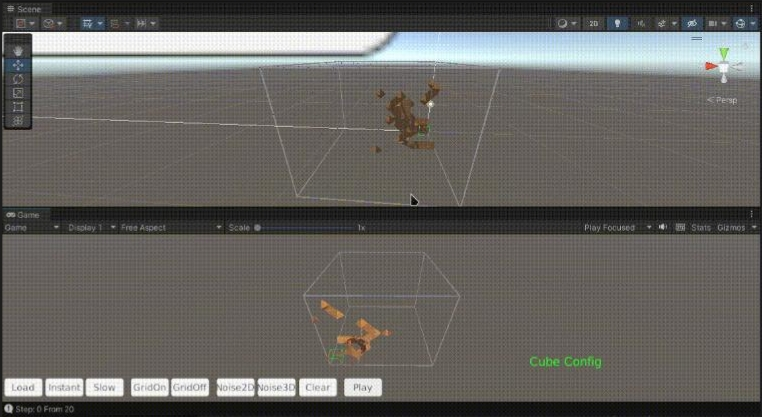
\includegraphics[width=0.9\textwidth]{tumor.jpg}
  \caption{Ejemplo de la simulaci\'on del crecimiento de un tumor en 3D en etapas tempranas. El c\'odigo fue desarrollado en Unity.}
  \label{fig:tumor}
\end{figure}

La creación de una herramienta para simular el crecimiento de un tumor con un autómata celular en cualquier órgano del cuerpo humano es un avance significativo en el campo de la modelación y simulación de sistemas biológicos. Esta herramienta proporciona un enfoque innovador y flexible para estudiar el crecimiento de los tumores, lo cual tiene importantes implicaciones tanto en la investigación básica como en la clínica.

La capacidad de cargar configuraciones específicas y ajustar, agregar o eliminar parámetros que influyen en el realismo de la simulación permite adaptar el modelo a diferentes escenarios y condiciones. Esto hace que la herramienta sea altamente versátil y aplicable a una amplia gama de situaciones y tipos de tumores.

El uso de autómatas celulares para simular el crecimiento del tumor proporciona una representación detallada y dinámica del proceso. Los autómatas celulares son especialmente adecuados para este tipo de modelado, ya que permiten representar de forma precisa y realista la interacción entre las células y su entorno, así como los cambios que ocurren en el tiempo~\cite{2}.\\

¿Cuánto progreso se ha hecho hasta ahora?
\begin{itemize}
    \item Se ha implementado la carga y uso de parámetros para la simulación.
    \item Se ha implementado el motor para simular el crecimiento de un tumor en órganos pequeños. 
    \item Se ha visualizado y analizado el gráfico de células con sus conexiones.\ref{fig:3d_graph}
    \item Se ha visualizado el tamaño que tomará el tumor durante la simulación.
    \item Se ha implementado el código para renderizar la forma que tendrá el tumor.\ref{fig:tumor}
\end{itemize}

¿Cuál será el enfoque en las próximas etapas? 
\begin{itemize}
    \item Mejorar todo lo anterior, por ejemplo, mejorar la implementación de la renderización 3D utilizando Marching Cubes para obtener caras y triángulos más suaves.
    \item  Implementar cambios entre estados siguiendo los detalles encontrados en la literatura.
    \item Implementar algoritmos eficientes para procesar grandes cantidades de células y sus conexiones, estamos hablando de millones de ambos.
    \item Agregar técnicas de Inteligencia Artificial y Aprendizaje Automático para obtener mejores aproximaciones a la realidad.
\end{itemize}

Finalmente, la visualización en 3D del crecimiento de un tumor utilizando la técnica de Marching Cubes puede proporcionar una herramienta valiosa para los profesionales de la salud para entender mejor la dinámica del crecimiento del tumor y desarrollar estrategias de tratamiento más efectivas.

%%%%%%%%%%%%%%%%%%%%%%%%%%%%%
%%%%%%%%%%%%%%%%%%%%%%%%%%%%%

\section*{Recomendaciones}

Luego de obtener varios resultados en el presente estudio se sugieren varias recomendaciones dirigidas a mejorar el modelo y potenciar posibles direcciones para investigaciones futuras y aplicaciones prácticas:
\begin{itemize}
    \item \textbf{Mejora de las técnicas de visualización}: Aunque el uso de la técnica de Marching Cubes para la renderización en 3D ya proporciona una representación detallada y precisa de los tumores, se deben explorar técnicas de visualización más avanzadas para mejorar la precisión y la capacidad de detalle de la simulación. Esto podría permitir una comprensión aún más profunda del crecimiento y propagación del cáncer.
    \item \textbf{Incorporación de más parámetros en la simulación}: La simulación podría mejorarse aún más incorporando más parámetros, como la genética del paciente, el tipo y etapa del cáncer, y otros factores de salud. Esto podría permitir una simulación más precisa y personalizada del crecimiento tumoral.
    \item \textbf{Uso de la simulación para la educación y la formación}: La simulación podría utilizarse como herramienta de enseñanza para los estudiantes de medicina y los profesionales de la salud, ayudándoles a comprender mejor cómo se desarrolla y se propaga el cáncer. También podría utilizarse para la formación de pacientes y sus familias, proporcionándoles una comprensión visual de lo que está ocurriendo en el cuerpo.
    \item \textbf{Investigación adicional sobre el uso de la Inteligencia Artificial y el Aprendizaje Automático}: Como se mencion\'o anteriormente, se planean incorporar técnicas de Inteligencia Artificial y Aprendizaje Automático en futuras versiones de la herramienta. Se cree que esto podría permitir predecir con mayor precisión cómo se desarrollará y se propagará un tumor. Se recomienda que se realicen más investigaciones en esta área.
    \item \textbf{Promoción de la adopción de la herramienta por parte de los profesionales de la salud}: Para maximizar el impacto de la herramienta, sugerimos trabajar para promover su adopción por parte de los profesionales de la salud. Esto podría implicar la realización de demostraciones y talleres, la creación de materiales de capacitación y la colaboración con hospitales y clínicas.
    
\end{itemize}
%%%%%%%%%%%%%%%%%%%%%%%%%%%%%
%%%%%%%%%%%%%%%%%%%%%%%%%%%%%

\section*{Ap\'endices}

Para desarrollar este trabajo se utilizaron las siguientes herramientas:
\begin{itemize}
    \item En la parte de la generaci\'on de la simulaci\'on, C\# en su versi\'on de .net7.0.
    \item En la parte visual para visualizar las c\'elulas y sus conexiones en determinadas regiones Python en su versi\'on 3.11 con Streamlit y otras dependencias.
    \item En la parte visual para renderizar el tumor, Unity en su versi\'on 2021.3.28f1.
\end{itemize}

%%%%%%%%%%%%%%%%%%%%%%%%%%%%%
%%%%%%%%%%%%%%%%%%%%%%%%%%%%%


\section*{Referencias bibliográficas}
\label{Nada}
\begin{flushleft}

\begin{thebibliography}{99}

\bibitem{1} Cirne, M. A.; Pedrini, H. Marching cubes technique for volumetric visualization accelerated with graphics processing units. Journal of the Brazilian Computer Society, vol. 19, pages 223-233, 2013. Available at: https://journal-bcs.springeropen.com/articles/10.1007/s13173-012-0097-z.

\vskip 0.2cm
\bibitem{2} Deutsch, A.; Maini, P.; Dormann, S. Cellular Automaton Modeling of Biological Pattern Formation: Characterization, Applications, and Analysis. \textit{Modeling and Simulation in Science, Engineering and Technology}. Birkhauser Boston, 2007.

\vskip 0.2cm
\bibitem{3} Guinot, V. Modelling using stochastic, finite state cellular automata: rule inference from continuum models. \textit{Applied Mathematical Modelling}, 26:701–714, 2002.


\vskip 0.2cm
\bibitem{4} Kansal, A.; Torquato, S. Simulated brain tumor growth dynamics using a three-dimensional cellular automaton. \textit{Journal of Theoretical Biology}, 203:367–382, 2000.

\vskip 0.2cm
\bibitem{5} Lorensen, W. E.; Cline, H. E. Marching cubes: A high-resolution 3D surface construction algorithm. ACM SIGGRAPH Computer Graphics, vol. 21, no. 4, pp. 163-169, 1987. Available at: https://people.eecs.berkeley.edu/~jrs/meshpapers/LorensenCline.pdf.\\

\vskip 0.2cm
\bibitem{6} Ruanxiaogang, H. A simple cellular automaton model for tumor-immunity system. In \textit{Robotics, Intelligent Systems and Signal Processing, 2003. Proceedings. 2003 IEEE International Conference on}, 2.

\vskip 0.2cm
\bibitem{7} Viera Barredo, D. Universidad de La Habana, Facultad de Matemática y Computación. Departamento de Matemática. Autómata celular estocástico en redes complejas para el estudio de la invasión, migración y metástasis del cáncer. Asesores: Reinaldo Rodríguez Ramos, Rubén Interián, Ariel Ramírez Torres, Rocío Rodríguez Sánchez. Undergraduate thesis. June, 2019. Available at: https://raw.githubusercontent.com/Krtucho/cellular\_automata/main/docs/darien-tesis.pdf

\vskip 0.2cm
\bibitem{8} Visutsak, P. Marching Cubes and Histogram Pyramids for 3D Medical Visualization. Journal of Imaging, vol. 6, 2020. Available at: https://ncbi.nlm.nih.gov/pmc/articles/PMC8321043 and https://api.semanticscholar.org/CorpusID:225446991.

\vskip 0.2cm
\bibitem{9} Watts, D. J. \& Strogatz, S. H. Collective dynamics of small-world networks. \textit{Nature}, 393:440–442, 1998.

\end{thebibliography}

%Livro com até 3 autores:

\end{flushleft}

\newpage
\section*{Anexos}

\begin{figure}[h]
  \centering
  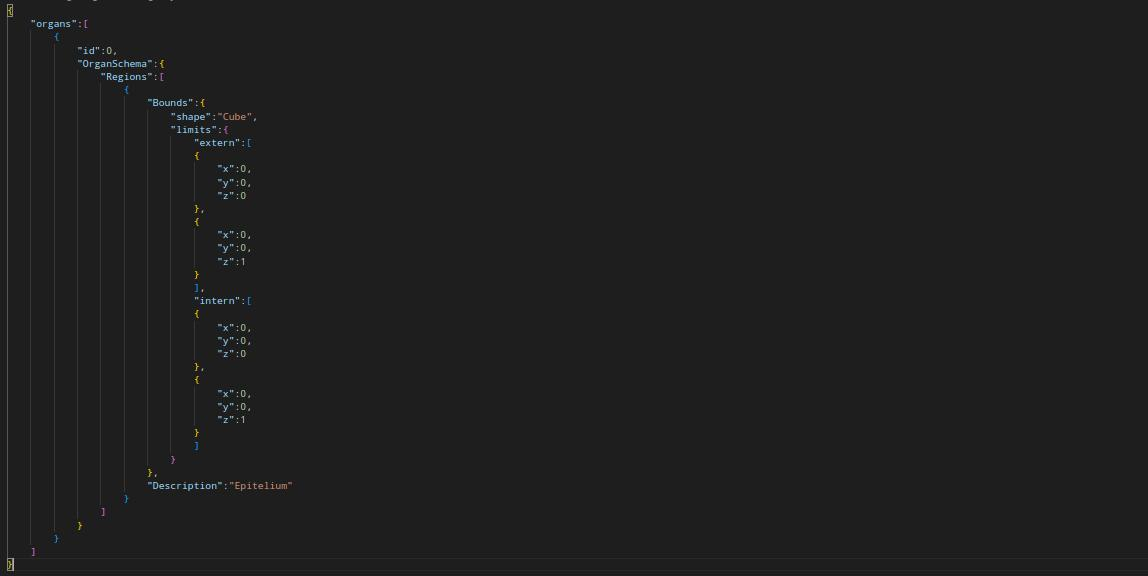
\includegraphics[width=0.9\textwidth]{organ_config.jpg}
  \caption{Ejemplo de archivo de configuraci\'on de \'organos. Se indica la forma que tendr\'a esta regi\'on indic\'andola en "shape".}
  \label{fig:organ_config}
\end{figure}

\begin{figure}[h]
  \centering
  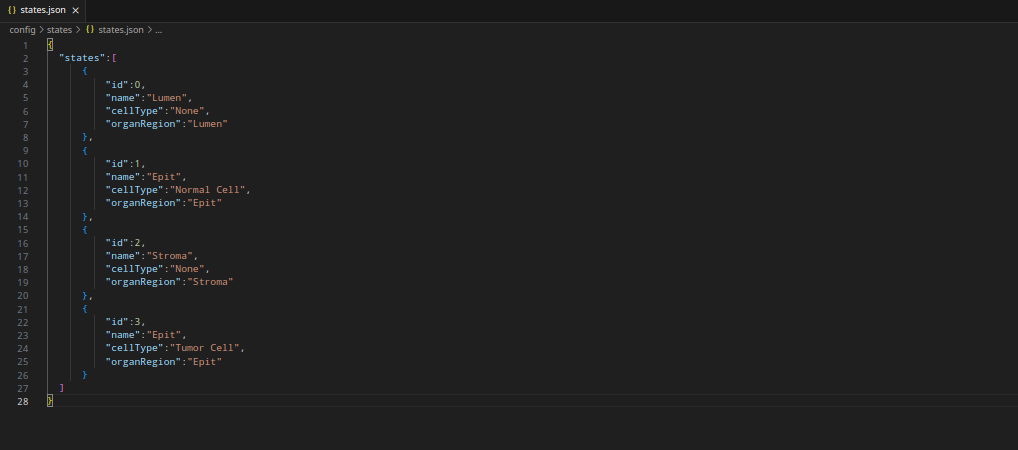
\includegraphics[width=0.9\textwidth]{json.png}
  \caption{Ejemplo de archivo de configuraci\'on de los estados que tendr\'a nuestro aut\'omata celular.}
  \label{fig:json}
\end{figure}

\begin{figure}[h]
  \centering
  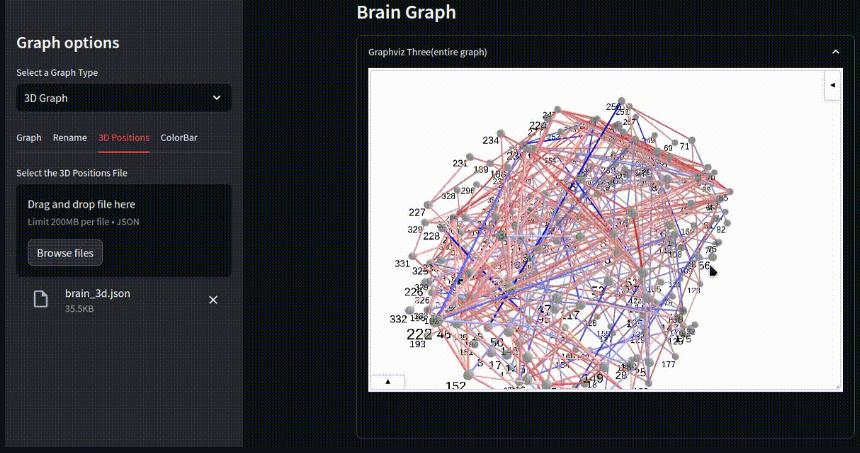
\includegraphics[width=0.9\textwidth]{3d_graph.jpg}
  \caption{Visualización de las células y las conexiones entre las mismas.}
  \label{fig:3d_graph}
\end{figure}

\end{document}
